\documentclass{standalone}
\usepackage{tikz}
\usepackage{tabu}
\usepackage{enumitem}

\begin{document}

\begin{tikzpicture}

\node {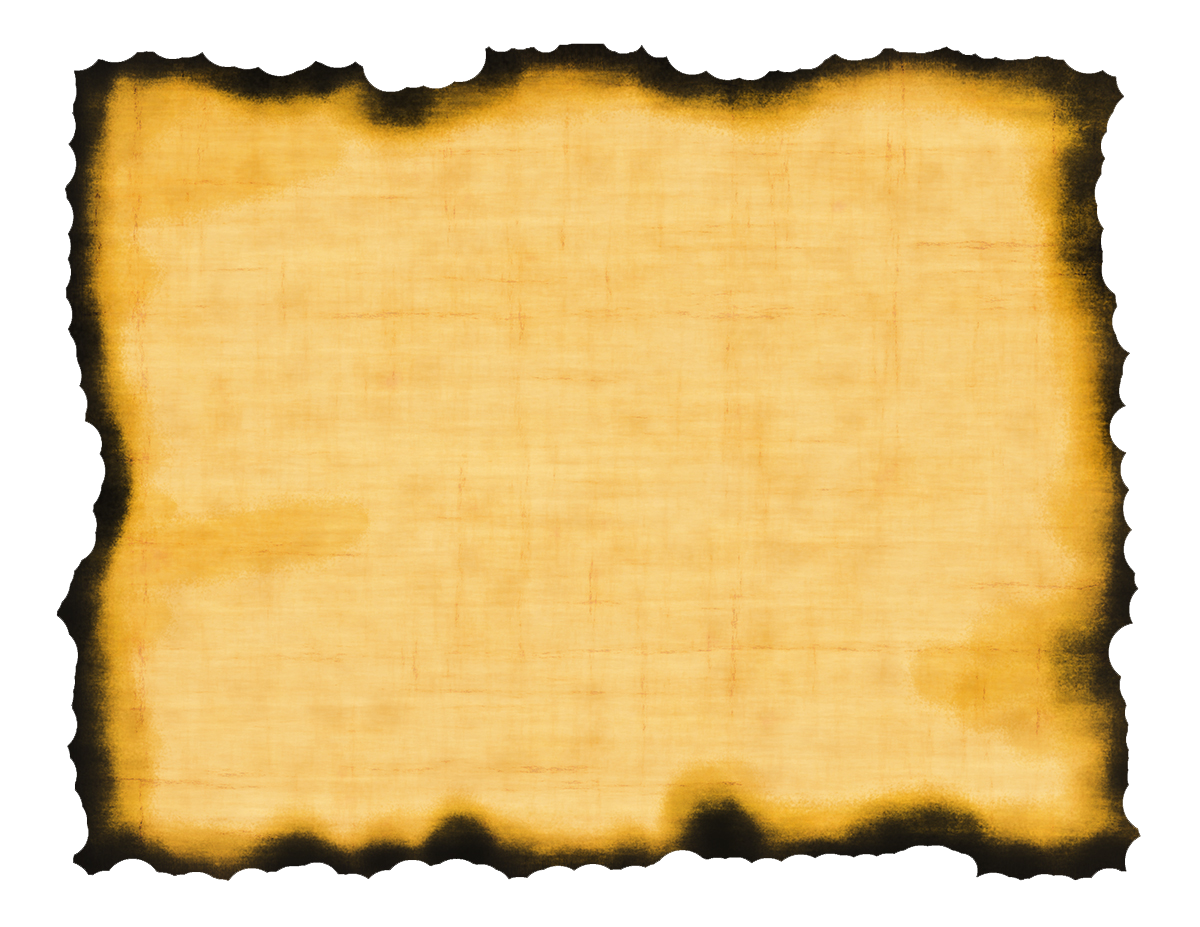
\includegraphics[width=400bp]{papiro.png}};
\node [rectangle]{\parbox{300bp}{
Há dois baús escondidos, um deles carregado com um tesouro. Para localiza-los, você deve seguir o mapa e estas instruções.

\begin{enumerate}[label=\arabic*.,topsep=.5em]
\setlength\parskip{.1em}
\setlength{\baselineskip}{10pt}
\item Use a faixa vermelha como unidade para descobrir a localização dos baús.
\item Os baús estão enterrados no caminho em destaque, alinhados com a palmeira imperial e com a pedra.
\item No mapa, os pontos que marcam os locais em que os baús estão enterrados ficam a $\frac{5}{6}$ e a $\frac{5}{8}$ da unidade, a partir da palmeira. A chave do baú com o tesouro está enterrada a $\frac{13}{8}$ da unidade a partir da palmeira.
\item O baú com o tesouro está mais distante da palmeira.

\end{enumerate}}};

\end{tikzpicture}

\end{document}